\documentclass[onecolumn,12pt]{aastex62}
\pdfoutput=1 %for arXiv submission
\usepackage{amsmath,amstext} %math symbols and text
\usepackage[T1]{fontenc} %font encodingd, accents
\usepackage{apjfonts} %use ApJ's fonts (comes with the .cls file)
\usepackage[figure,figure*]{hypcap} %nice figure captions
\usepackage{comment} %comment out blocks of text
\usepackage{color} %use colors, great for commenting
\usepackage{verbatim} %to insert latex code without executing it

%It's often useful to define shortcuts for things
\newcommand{\ha}		{\mbox{\rm{H}$\alpha$}}
\newcommand{\hb}		{\mbox{\rm{H}$\beta$}}
\newcommand{\hg}		{\mbox{\rm{H}$\gamma$}}
\newcommand{\kms}		{\mbox{km\,s$^{-1}$}}
\newcommand{\HI}        {\mbox{\rm H{\small I}}}
\newcommand{\HII}       {\mbox{\rm H{\small II}}}
\newcommand{\git}	    {{\fontfamily{cmtt}\selectfont git}}
\defcitealias{levy18}{Paper I}
\newcommand{\cta}		{\citetalias}
\newcommand{\cpa}		{\citepalias}
\newcommand{\blue}      {\textcolor{blue}}

%if a command with that name already exists, you can redefine it (use this carefully!)
\renewcommand{\HI}      {\hi}

% Define a short title and short authors for aastex62
%\shorttitle{LaTeX Examples}
%\shortauthors{Levy et al.}

\begin{document}
%The placement of the \begin{document} command matters

\title{LaTeX Examples with Overleaf for ASTR 695}

\author{Rebecca C. Levy}
\affiliation{University of Maryland}
\author{Iman Example}
\affiliation{University of Maryland}
\affiliation{NASA Goddard Space Flight Center}
\email{rlevy.astro@gmail.com}

\begin{abstract}
This document is an example of how to use LaTeX - and specifically Overleaf - for scientific papers.
\end{abstract}

%make article keywords for aastex62
%\keywords{keyword1 --- keyword2 --- keyword3}

%add a linked table of contents to easily navigate this guide
\tableofcontents
\clearpage

\section{Introduction}
\label{sec:intro} %it's a good practice to label all your sections, subsections, figures, tables, and equations so you can easily reference them in-text

LaTeX is a flexible word processor used for scientific publications. Like anything, there is a learning curve to getting started, but the payoff over another word processor (like Word or Pages) is huge. There are three main areas where I think LaTeX really shines:
\begin{enumerate}
\itemsep0em 
    \item Typing equations and mathematical symbols
    \item Automatically referencing citations, figures, tables, sections, etc in text
    \item Flexibility in float (i.e. figure or table) placement.
\end{enumerate}
Moreover, most plotting tools (matplotlib, Matlab, etc) have LaTeX interpreters, so you can use LaTeX-style fonts and symbols in your plots using LaTeX's syntax. 

There are many ways to use LaTeX, such as:
\begin{itemize}
\itemsep0em 
\item In the cloud:
	\begin{enumerate}
	\item Overleaf: \url{www.overleaf.com}
	\item ShareLaTeX: \url{www.sharelatex.com} (newly merged with Overleaf)
	\end{enumerate}
\item On your computer:
	\begin{enumerate}
	\item TeXShop: \url{https://pages.uoregon.edu/koch/texshop} (my personal favorite because I like IDEs)
    \item TeXworks: \url{http://www.tug.org/texworks}
    \item MacTeX: \url{http://www.tug.org/mactex}
    \item MiKTeX: \url{https://miktex.org/} (what I used when I had a Windows machine)
    \end{enumerate}
\end{itemize}

In the following sections, we'll go over the different parts of a LaTeX document.

\textcolor{red}{\textbf{Disclaimers:}} I am not a LaTeX expert! This is what works for me. I do a \textit{lot} of Googling. This guide is in no way complete. See the source code for examples of some things I won't explicitly go over. To see a complete example, see \url{http://journals.aas.org/authors/aastex/aasguide.html} or \url{https://www.overleaf.com/read/prpfjsqmgnqm}. The latter is a paper I wrote that has some neat features that I struggled with, like tables input from uploaded files, sideways tables, multi-page tables, and multi-panel figures masquerading as tables (noticing a theme yet?). I'm going to do a decent amount of ``self-citing'' in this guide. This is not because I think I have the best LaTeX code ever (certainly not), it's just what I have access to and permission to distribute.

\subsection{Basics of LaTeX}
\label{ssec:latexbasics}
To get started, I highly recommend consulting/ bookmarking the LaTeX Wikibook: \url{https://en.wikibooks.org/wiki/LaTeX}. 

There are different LaTeX compilers. Generally, you won't need to worry about them and can use pdfLaTex (which is usually the default)\footnote{If you're using a non-standard font or one from a font file on your machine, you might have to use LuaLaTex. This is the only situation I've had to change compilers, and the error message told me how to fix the problem.}. 

LaTeX has some special symbols that it uses internally. These include (but are not limited to): \% \& \_ \{ \} \$ \# \textbackslash. To insert them as a symbol in a document, use \verb|\%|. The exception is \textbackslash\ for which you use \verb|\textbackslash|.

To get quotation marks that look nice, you need to use \verb|``''|, which will produce ``a quote with nice quotation marks''. If instead you use the normal double quotation mark key, you'll get "a quote with not as nice quotation marks." Depending on your compiler, these will sometimes look even worse (e.g. ''This makes my skin crawl'').

To comment out a single line, use \%\ (everything in that line after \% will be commented out). To comment out a block of text, you can use \%\{...\} (everything within the brackets will be commented out). If, however, the block of text has line breaks in it, you'll need to use \verb|\begin{comment}...\end{comment}| from the comment package. 
%Here is a line I've commented out
%{Here's block of commented text}
\begin{comment}
And here is a block of commented text with line breaks
Blah
Blah
Blah
\end{comment}

Here is a list of common accents to add to letters. Replace the letter in brackets with whatever letter you want.
\begin{itemize}
\itemsep0em 
    \item \'{a}: \verb|\'{a}|
    \item \`{e}: \verb|\`{e}|
    \item \"{u}: \verb|\"{u}|
    \item \~{n}: \verb|\~{n}|
    \item \^{o}: \verb|\^{o}|
\end{itemize}

\noindent\makebox[\columnwidth][c]{
    \begin{minipage}{0.9\columnwidth}
        \noindent\blue{\hrulefill}\par
        \blue{\textbf{Your turn:} Practice typing some symbols and words/names with accents.}\\
        \blue{Ex: Fran\c{c}ois bought a shirt for \$5. It was 80\% off.}\\
        
        \noindent\blue{\hrulefill}\par
    \end{minipage}}\\

There are several ways to start a new line in LaTeX. One is to hit return twice (as I've been doing so far). Another is to use \verb|\\| at the end of a line:\\Here's a new line (notice there's no indent with this method). A third way is to use \verb|\newline|:\newline but this is rare.  To get a blank line between paragraphs, use two returns and \verb|\\|\\

so you get a gap like this.

\noindent Another useful formatting command is \verb|noindent|, which undoes the automatic indentation. \verb|\clearpage| starts a new page, which is especially useful when writing proposals with strict page limits for each section.

\subsubsection{Math Mode}
\label{sssec:mathmode}
To type equations and access more symbols, you'll use math mode. This is where LaTeX \textit{shines}. It takes a little while to get used to, but once you do, it's very efficient (and much better than Word). There are a few ways to do this. For inline text, bracket your mathematical expression with \verb|$...$|: $4\times10^{6}~{\rm M}_\odot$ or $y_{\rm{final}} = \int_0^\infty \log(x)\sin(x)dx$ (Be sure to look at the source code for some of the special characters.) If you want an equation to have its own line, use \verb|$$...$$|:
$$ V_{\rm Persic}(x) = V(R_{\rm opt})\Bigg \{\Big[0.72+0.44\log(L_B/L_{B*})\Big]\frac{1.97x^{1.22}}{(x^2+0.78^2)^{1.43}}+1.6\exp{\Big[-0.6(L_B/L_{B*})\Big]\frac{x^2}{x^2+1.5^2(L_B/L_{B*})^{0.4}}} \Bigg\}^{1/2} {\rm km\ s^{-1}} $$
Yet a third way to use math mode is \verb|\begin{equation}...| \verb|\end{equation}|. This has the added bonus of automatically numbering your equations and allowing you to reference them in the text:
\begin{equation}
\label{eq:persicprofile}
     V_{\rm Persic}(x) = V(R_{\rm opt})\Bigg \{\Big[0.72+0.44\log(L_B/L_{B*})\Big]\frac{1.97x^{1.22}}{(x^2+0.78^2)^{1.43}}+1.6\exp{\Big[-0.6(L_B/L_{B*})\Big]\frac{x^2}{x^2+1.5^2(L_B/L_{B*})^{0.4}}} \Bigg\}^{1/2} {\rm km\ s^{-1}}
\end{equation}
Equation \ref{eq:persicprofile} gives the form of the Universal Rotation Curve \citep{persic96} (see Section \ref{sec:referencing} for more about referencing).

Math mode also gives you Greek letters: $\alpha,\ \Delta,\ \delta$. For a mostly complete list of symbols in LaTeX, see \url{https://artofproblemsolving.com/wiki/index.php/LaTeX:Symbols}. Two symbols that aren't on that site that I use somewhat frequently are $\gtrsim$ (\verb|\gtrsim|) and $\lesssim$ (\verb|\lesssim|).

To use the regular font style in math mode, use the command \verb|{\rm}| or \verb|\textrm{}|. You might want your text (in a variable name for example) to look like $V_{\rm rot}$ or $V_{\textrm{rot}}$ instead of $V_{rot}$ (note the different bracket placements in the source code). There is also the `\verb|\mathcal{}| option, which gives you script capital letters such as $\mathcal{L} {\rm\ and\ } \mathcal{F}$. For lowercase script letters, you'll need to look through some other packages, but the commonly used $\ell$ is \verb|$\ell$|.

To insert a space in math mode, you'll need to use \textbackslash\ between characters (see the example in the source code with the Greek letters above). Note this can also be used outside math mode to insert a space. Sometimes spacing with symbols in general can be weird, especially if you're using one of the shortcuts you made (see Section \ref{ssec:shortcuts}). Here I'm using the shortcut I made for \ha\ where I have to type \verb|\ha\ | or \ha would run into the next word like this. You can also insert a small space between characters using \verb|\,| or \verb|~|. This looks especially nice for galaxy names (NGC253 v. NGC\,253 v. NGC~253 v. NGC 253) and units (5pc v. 5\,pc v. 5~pc v. 5 pc). \\

\noindent\makebox[\columnwidth][c]{
    \begin{minipage}{0.9\columnwidth}
        \noindent\blue{\hrulefill}\par
        \blue{\textbf{Your turn:} Practice typing some expressions that use fractions, special characters, exponents, regular text, etc.}\\
        \blue{${\rm Ex:}\ \frac{-\hslash^2}{2m}\nabla^2\Psi(r)+V(r)\Psi(r) = E\Psi(r)$}\\
        
        
        \noindent\blue{\hrulefill}\par
    \end{minipage}}\\

\subsection{Basics of Overleaf}
\label{ssec:overleafbasics}
Overleaf is a wonderful, flexible, cloud-based LaTeX editor. Overleaf and ShareLaTeX recently merged, and  Overleaf v2 is new (this is my first time using it). Overleaf has free and paid versions. I've been fine using the free version so far. Documents are organized by projects, which contain all the supporting documents, images, etc that get complied into the final document. You can easily add, delete, or replace associated files from the file-tree to the left. Overleaf has wonderful find and replace capabilities (not sure where the button went in v2 but Cmd+f on a Mac works). Finally, if you \textit{really} don't like the source code approach to LaTeX, there is a Rich Text editor, but other LaTeX editors may not have this feature, and you'll still have to use some of the source code commands.

I use Overleaf almost exclusively because I can share documents with my collaborators who can see real-time updates. No more emailing old versions back and forth: the same link always works. You can also easily give different people read or write privileges using the ``Share'' button, so \textit{that} collaborator doesn't mess up all the formatting or accidentally delete everything. And speaking of deleting everything, see Appendix \ref{app:backup} for how to easily backup your entire project to your computer. 

You can quickly navigate to the same place in the source code as the PDF view (and vice-verse in v2). Simply double click on a location in the PDF view and it will take you to that location in the source code. In v2, you can also use the arrows in the center of the page to jump to the current location in either view.

To compile your source code, click the green ``Recompile'' button. My preference is to have Overleaf auto-compile (click the arrow on the Recompile button and turn Auto Compile on). However, I'll admit that this may be annoying for some people, especially if multiple people are editing the document. When there are errors with your document (or other attached files), the ``logs and outputs'' icon (piece of paper to the right of ``Recompile'') will have a red badge showing the number of errors. Click on it, and it will (try to) tell you what and/or where the problem is. If there's a yellow icon, there's a warning somewhere. Icons will also show up on the line that's throwing the error or warning in the source code or other file.


\section{Preamble}
\label{sec:preamble}
The preamble of a LaTeX document is where you define the kind of document you're working on, load any packages you'll need, define shortcuts and aliases, and give the title and author information.

\subsection{Document Class}
\label{ssec:docclass}
The general document class is ``article''. For this example I'm using aastex62 (AASTeX v6.2), which is the template for submissions to the Astrophysical Journal\footnote{More info, downloads, and examples at \url{http://journals.aas.org/authors/aastex/aasguide.html}.}. Most other journals will have their own templates as well. If you're using a template, you'll need the associated class and style files (see aastex62.cls and apjfonts.sty in the file-tree to the left). I find the preformatting of a template nice for most things. There are some options you can change, such as the number of columns and fontsize (e.g. \verb|\documentclass[twocolumn,10pt]{aastex62}|).

Sometimes, however, the templates may not flexible enough if you're not writing a journal article. For more flexibility, I use the article class, but there's a lot more setup required. For an example of an article, see my \href{https://www.overleaf.com/read/kvjqzkbkjdnh}{draft thesis proposal}. Here, I wanted some flexibility in how the title page was formatted. Note the increased number of packages loaded and section formatting.

There are many kinds of documents you can produce with LaTeX's pre-defined document classes such as r\'esum\'es, presentations, reports, and books. Overleaf has a library of templates for various journals and document classes to get you started.

\subsection{Packages}
\label{ssec:packages}
There are a number of packages you can load into LaTeX (similar to loading modules in Python). When using a template like aastex62, some packages are pre-loaded while others may not be compatible. For example, the commonly used package ``graphicx'' is pre-loaded in aastex62, while ``caption'' is incompatible. For a basic article, take a look at my \href{https://www.overleaf.com/read/kvjqzkbkjdnh}{draft thesis proposal} for the packages I have loaded. This is why I start with a template like aastex62 if I can.

\subsection{Shortcuts and Aliases}
\label{ssec:shortcuts}
Shortcuts are very useful for commands you'll be typing a lot. For example, I can type \verb|\ha| rather than \verb|H$\alpha$| for \ha. This is also nice for commands with long names (example shown in Section \ref{sssec:citeref}). 

\subsection{Title and Authors}
\label{ssec:authors}
Before the title, there is the \verb|\begin{document}| command (the \verb|\end{document}| command goes at the very end of the document). The title of your document goes in the \verb|\title{}| command. Overleaf automatically uses the title of the document as the title in your Projects list, but you can change this from the Projects list. For the authors in aastex, a single author can have multiple affiliations, and each co-author gets their own \verb|\author{}| command, as shown. The \verb|\email{}| command is specific to aastex and gives the email of the corresponding author. 

\subsection{Abstract}
\label{ssec:abstract}
Where the abstract for your paper goes. This is a specially formatted section, both in aastex and for articles in general, defined by the \verb|\begin{abstract}..\end{abstract}| environment. It spans both columns of a twocolumn document.


\section{Main Body}
\label{sec:mainbody}
Where everything else goes! Below are some commands for section formatting.

\subsection{This is a subsection}
\label{ssec:ssec}
Here is some text in a subsection. Note that the section numbering and text styles are determined by this template. If you want more customization, use \verb|\documentclass{article}|.

\subsubsection{This is a sub-subsection}
\label{sssec:sssec}
Here is some text in a sub-subsection.

\paragraph{Paragraph} Here is some text in a labeled paragraph.

For an example Appendix, see Appendix \ref{app:appendices}.

\section{Referencing}
\label{sec:referencing}
This is another place where I think LaTeX really shines. Referencing sections, appendices, figures, tables, and equations within your document is seamless and painless. Referencing bibliographic citations is slightly more work up front, but the payoff is enormous.  

\subsection{Referencing Objects in Text}
\label{ssec:ref}
Referencing sections, appendices, figure, tables, and equations in your document is easy. Use the \verb|\label{key}| command to label the object to be referenced. You can see examples throughout where I've done this. I try to give them useful keys that also indicate what kind of object they are (i.e. fig for figure, tab for table, sec for section, etc). Get in the habit of labeling everything, even if you never reference it (although you should reference all your tables and figures). Then when you're ready to reference your object, simply use \verb|\ref{key}|. Done. Easy. No need to update every instance of Figure 1 if you add a figure before it; LaTeX takes care of it for you. 

\subsection{Bibliography}
\label{ssec:bibliography}
Another reason I prefer to use a template like aastex is for the bibliography capabilities. The best bibliography package for LaTeX is ``natbib'', which is automatically included in aastex. natbib integrates fairly seamlessly with \href{https://ui.adsabs.harvard.edu/}{SAO/NASA ADS} and bibliography preparation services like BibDesk. Using natbib on it's own can lead to some consternation, but there's a lot of help online. I'll refer you to this excellent article about using natbib and other reference styles: \url{https://www.sharelatex.com/learn/Bibliography_management_with_natbib}. Even if you're not using aastex, you can still use the aastex bibliography style file (yahapj.bst). \citep{bolatto17}

To make the bibliography, there are two lines that go where you want the bibliography to appear. The first is \verb|\bibliographystyle{stylename}|. For ApJ citation style, use \verb|\bibliographystyle{yahapj}| and be sure that yahapj.bst is in the file-tree. For other common citation styles, see \url{https://www.sharelatex.com/learn/Natbib_bibliography_styles}. The line is \verb|\bibliography{bibfile}|, where bibfile is the name of the .bib file where the full citation information is stored (see Section \ref{sssec:bibfile}). The References section will only show those references cited in the text. In other words, if you have ten references in your bibfile, but only cite two of them, only those two that have been cited will appear in the References section.

\subsubsection{Creating the Bibfile}
\label{sssec:bibfile}
This is largely up to personal preference. Some people use software like BibDesk. Personally, I copy the bibliography info from ADS into the bibfile manually (and I cite as I write to save myself pain and suffering later). From ADS, simply copy the BibTeX formatted citation info into the .bib file. I usually rename the citation key with something I can remember easily (e.g. lastnameYY). Check out references.bib in the file-tree to see some examples. 

\subsubsection{Citing References in Text}
\label{sssec:citeref}
Once your bibfile is set up, you're ready to cite things! There are two commands you'll need: \verb|\citet{}| and \verb|\citep{}|. \verb|\citet| is used to cite things in the text: \citet{levy18} show that blah causes blah. \verb|\citep| is used for parenthetical citations: Blah causes blah \citep{levy18}. If you're citing more than one reference, they get grouped into the same citation command: \citep{levy18,persic96}. You can also add additional text into the citation using \verb|\citep[][]{}|: \citep[e.g.][]{levy18}.

If two (or more) citations have the same shortened author list and year, LaTeX will automatically label them a, b, etc chronologically based on the publication info given in the bibfile: \citet{kennicutt98a} and \citet{kennicutt98b}, \citet{kennicutt98a,kennicutt98b}, or \citep{kennicutt98a,kennicutt98b}. (Also check out how spiffy this looks in the list of references.)


Here is an example of using a citation alias. For example, rather than referring to Levy et al. 2018 in my next paper, I'd like it to show up as ``Paper I''. I can create an alias for that reference using \verb|\defcitealias{paperkey}{Paper I}|. Then, to reference that citation alias in text, I would use \verb|\citetalias{paperkey}| or  \verb|\citepalias{paperkey}|. But those are long, and I'm lazy, so I'll alias them as \verb|\newcommand{\cta}{\citetalias}| and \verb|\newcommand{\cpa}{\citepalias}|. Then I can write: ``As shown in \cta{levy18}, blah blah blah'' and ``Blah blah blah \cpa{levy18}''. In the References section, the correct citation for Levy et al. 2018 is shown, and all the linking is correct. It's a good idea to use citation aliases sparingly so your readers can easily follow your paper and to define the alias the first time you use it: e.g. \citet[][hereafter \cta{levy18}]{levy18}.\\

\noindent\makebox[\columnwidth][c]{
    \begin{minipage}{0.9\columnwidth}
        \noindent\blue{\hrulefill}\par
        \blue{\textbf{Your turn:} Find an article to cite, add its info to the bibfile, and cite it.}
       
        Rebecca is really kool and it's nice that she's teaching us \citep{Richardson2000}.
        
        
        
        \noindent\blue{\hrulefill}\par
    \end{minipage}}

\section{Figures and Tables}
\label{sec:figuresandtables}
The amount of time you can spend \href{https://www.merriam-webster.com/dictionary/futz}{futzing} with figures and tables in LaTeX is infinite. Figures and tables are floats, which means they can move anywhere in the document. Usually, this is wonderful because LaTeX will find the best placement for your figure or table based on when it's referenced (see Section \ref{ssec:ref}). Other times, it means all your figures/tables end up at the end of the document for no apparent reason. There are also ways to force floats to appear exactly where you tell them to. However, this generally results in a lot of the aforementioned futzing, and I've found that letting some figures/tables float and fixing others generally doesn't end well. 

\subsection{Figures}
\label{ssec:figures}

The most basic way to insert a figure is:
\begin{verbatim}
    \begin{figure}[!h]
    \label{fig:umdastro}
    \centering
    
\includegraphics[width=0.2\textwidth]{umdastro.png}
    \caption{This is my figure.} 
    \end{figure}
\end{verbatim}
which produces:
\begin{figure}[!h]
    \label{fig:umdastro}
    \centering
    
\includegraphics[width=0.2\textwidth]{umdastro.png}
    \caption{This is my figure.} 
    \end{figure}

\begin{figure}
    \centering
    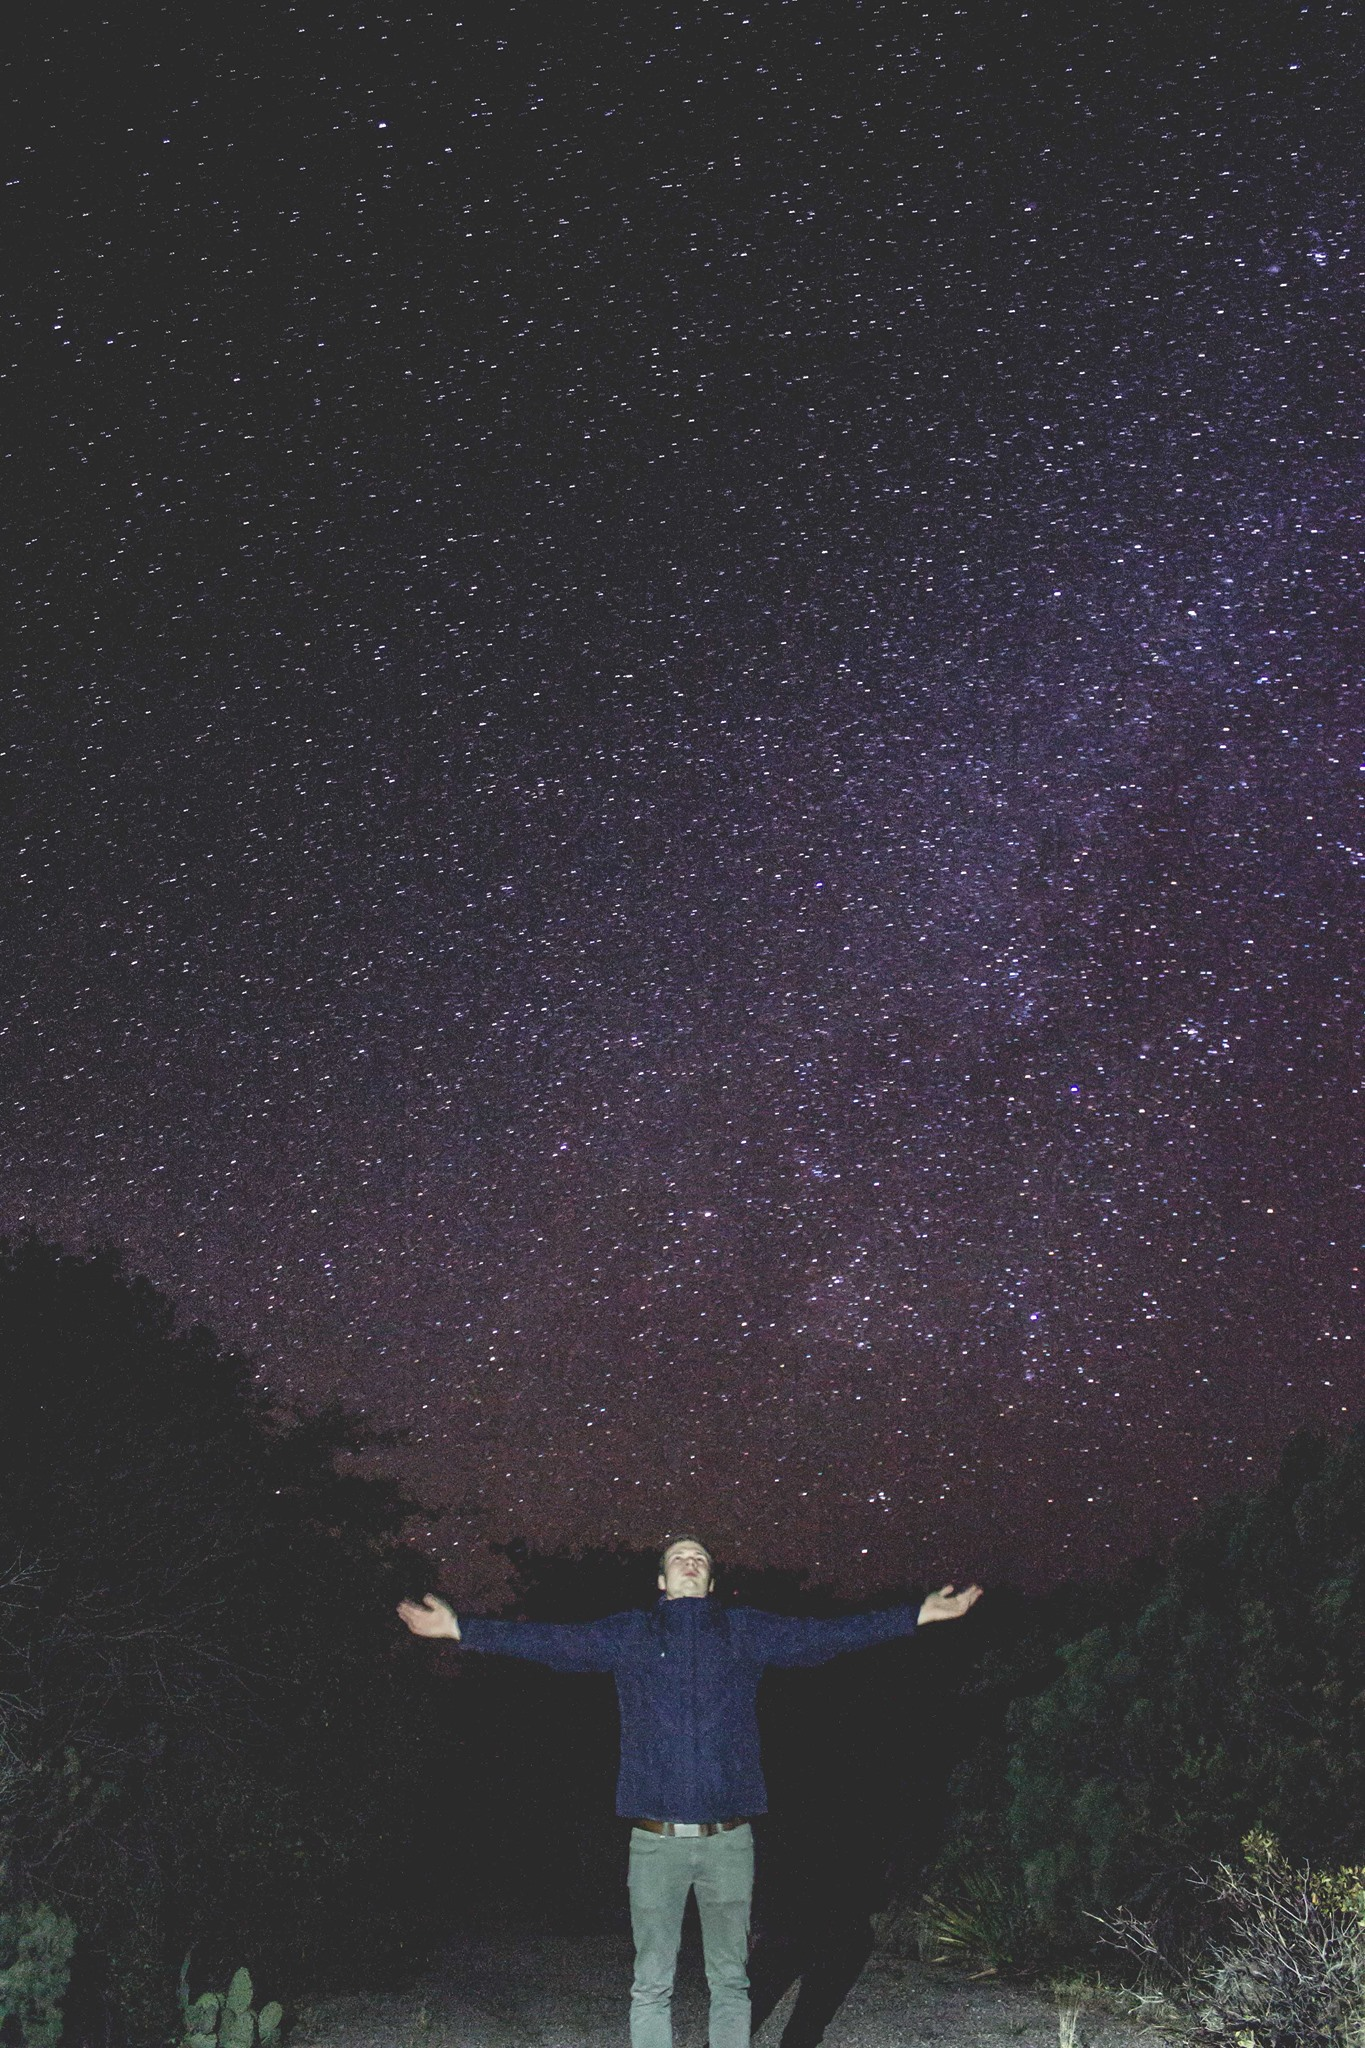
\includegraphics[width=0.2\textwidth]{Ben_with_stars_pic.jpg}
    \caption{hello world}
    \end{figure}
    
\begin{figure}
    \label{fig:RenStimpy}
    \centering
    
\includegraphics[width=0.2\textwidth]{Ren.jpg}
    \caption{Hello}
\end{figure}

\begin{figure}
    \label{fig:kitten}
    \centering
    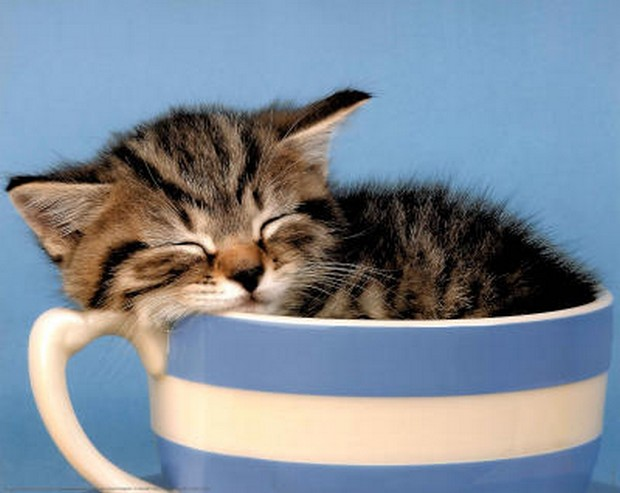
\includegraphics[width=0.5\textwidth]{kitten.jpg}
    \caption{This is a kitten in a cup. It's very cute and I hope you like it. Please treat kittens well.} 
    \end{figure}
    
To break this down a bit further, \verb|\begin{figure}[!h]| begins the figure environment with a location tag in []. \verb|h| means ``here'', and \verb|!| tells LaTeX to override its automatic figure placement. So \verb|[!h]| means that you want the figure to appear \textit{exactly} where you inserted it (Normally, this isn't a great idea.). Other location tags are \verb|t| (top), \verb|b| (bottom), and \verb|p| (on a page by itself). Note, you can stack location tags and LaTeX will use them in the order they appear: \verb|[htb]|. You can also use the figure environment without a location tag and leave LaTeX to is own devices. 

The main command to insert the figure is \verb|
\includegraphics[width=0.2\textwidth]{umdastro.png}| which defines what file to insert and how big to make it. If this were a two column document, the figure would be confined to a single column and would still only occupy 20\% of the column's width. If you want a figure to span both columns of a two column document, use the \verb|\begin{figure*}[]...\end{figure*}| environment, as shown in Figure \ref{fig:umdastro_wholepage}.\\

\begin{figure*}[t]
    \label{fig:umdastro_wholepage}
    \centering
    
\includegraphics[width=0.2\textwidth]{umdastro.png}
    \caption{This is my figure that spans the whole page width in a two column document.} 
    \end{figure*}
    
\noindent\makebox[\columnwidth][c]{
    \begin{minipage}{0.9\columnwidth}
        \noindent\blue{\hrulefill}\par
        \blue{\textbf{Your turn:} Insert an image!}\\
        
        
        \noindent\blue{\hrulefill}\par
    \end{minipage}}\\    
    
\subsubsection{Subfigures}  
\label{sssec:subfigures}
There are three ways to create subfigures:
\begin{enumerate}
\itemsep0em
    \item Make the subfigure outside of LaTeX. You can do this either in the programming language you used to make the figure in the first place or in PowerPoint, Photoshop, etc.
    \item Use the subcaption or subfig packages to access the subfigure environment. These aren't compatible with aastex, so I can't show an example, but see the following link: \url{https://en.wikibooks.org/wiki/LaTeX/Floats,_Figures_and_Captions#Subfloats}.
    \item Use \verb|\gridline| is aastex, which is very flexible. See the following link for more info: \url{http://journals.aas.org/authors/aastex/aasguide.html#new_figure_features}. You can do things like Figures \ref{fig:gridline1},  \ref{fig:gridline2}, and \ref{fig:gridline3}.
\end{enumerate}

\begin{figure*}
\label{fig:gridline1}
\centering
    \gridline{\fig{umdastro.png}{0.2\textwidth}{(a)}
    \fig{umd.png}{0.2\textwidth}{(b)}}
\caption{(a) UMD astro logo. (b) UMD logo.} 
\end{figure*}

\begin{figure}
\label{fig:gridline2}
\centering
    \gridline{\fig{umdastro.png}{0.2\textwidth}{(a)}}
    \gridline{\fig{umd.png}{0.2\textwidth}{(b)}}
\caption{(a) UMD astro logo. (b) UMD logo.} 
\end{figure}

\begin{figure*}
\label{fig:gridline3}
\centering
    \gridline{\fig{umdastro.png}{0.25\textwidth}{UMD Astro}
    \fig{umd.png}{0.25\textwidth}{UMD}}
     \gridline{\fig{testudo.jpg}{0.25\textwidth}{Testudo}
    \fig{marylandm.jpg}{0.25\textwidth}{The Maryland M}}
\caption{A bunch of logos.} 
\end{figure*}

\noindent\makebox[\columnwidth][c]{
    \begin{minipage}{0.9\columnwidth}
        \noindent\blue{\hrulefill}\par
        \blue{\textbf{Your turn:} Change the document to have two columns. Notice how the figures differ.}\\
        \noindent\blue{\hrulefill}\par
    \end{minipage}}\\ 

\subsubsection{Line Wrapping Around Figures}  
\label{sssec:wrapfig}

For some applications, you may want to wrap the text around a figure. This is especially useful when writing proposals with strict page limits. You'll need to use the wrapfig package. You can see examples in \href{https://www.overleaf.com/read/fwpbzsmdkhqy}{this recent proposal} of mine and at this link: \url{https://www.sharelatex.com/learn/Wrapping_text_around_figures}. The positioning requires a ton of futzing, so I wouldn't recommend this in general. 

\subsection{Tables}
\label{ssec:tables}
We've reached it, the skeleton in the LaTeX closet: tables. Here are two links about tables: \url{https://www.sharelatex.com/learn/Tables} and \url{https://en.wikibooks.org/wiki/LaTeX/Tables}. The main problem with tables in LaTeX is that they're tedious. 

To create a basic table,
\begin{verbatim}
    \begin{table}[h!]
    \centering
    \begin{tabular}{r | l c} 
    \hline\hline
    Col1 & Col2 & Col3 \\
    \hline
    1 & 6$\pm$1 & 8$^{+0.3}_{-0.2}$\\ 
    2 & 1 & 7 \\
    3 & 9 & 9 \\
    4 & 3 & 12 \\
    5 &  &  \\
    \hline
    \end{tabular}
    \caption{A basic table}
    \label{tab:table1}
    \end{table}
\end{verbatim}
which will produce:
\begin{table}[h!]
\centering
\begin{tabular}{r | l c} 
 \hline\hline
 Col1 & Col2 & Col3 \\
 \hline
 1 & 6$\pm$1 & 8$^{+0.3}_{-0.2}$\\ 
 2 & 1 & 7 \\
 3 & 9 & 4 \\
 4 & 3 & 12 \\
 5 &  &  \\
 \hline
\end{tabular}
\caption{A basic table}
\label{tab:table1}
\end{table}

\noindent Let's break down the syntax. Since tables are floats, you can again control their placement with \verb|[!htb]|. The \verb|{r l c}| controls the number of columns and their alignment (right, left, center). The | adds vertical lines. \verb|\hline| adds horizontal lines. Table entries are separated by \verb|&|, and new rows created with \verb|\\|. If the number of \verb|&| per line doesn't match the number of columns $-1$, LaTeX will throw an error, even if the cells are blank. 

Aastex has some unique (and very nice) table environments, which are described in detail at \url{http://journals.aas.org/authors/aastex/aasguide.html#tables}. These are automatically formatted in the correct style for publication in ApJ. They do have some unique syntax. They also have nice ways to rotate tables and make tables that span more than one page.

With few exceptions, you should never manually type a LaTeX table. You will regret it when you have to update the entries. The way around this is that you can insert other .tex files into the main LaTeX document using the \verb|\input{}| command. So my suggestion is that you script your LaTeX table generation to pull in whatever data will go in the table and write out the headers, footers, and correctly formatted data. I have scripts to do this in Matlab and Python if you'd like to see examples. There are also online code generators that will do this for you. An example input table is Table \ref{tab:persicparams} \citep[adapted from][]{levy18}, which is also an example of a aastex ``deluxetable''.

\begin{deluxetable}{ccccccc}
\tablecaption{Parameters for the Persic Profile Fits \label{tab:persicparams}}
\tabletypesize\footnotesize
\tablehead{
\colhead{Name} &\colhead{CO V(R$_{\rm opt}$)} & \colhead{CO $L_B$} & \colhead{CO R$_{\rm opt}$} & \colhead{H$\alpha$ V(R$_{\rm opt}$)} & \colhead{H$\alpha$ $L_B$}  & \colhead{H$\alpha$ R$_{\rm opt}$} \\
& (km/s) &\colhead{($\times10^8 \ L_{B\odot}$ )} & (arcsec) & (km/s) & \colhead{($\times10^8 \ L_{B\odot}$)} & (arcsec)}
\startdata
IC1199    &  168.7 & 2.8 & 7.2 & 181.7 & 8.8 & 14.4 \\
NGC2253    &  145.9 & 1.7 & 6.3 & 146.6 & 2.0 & 10.5 \\
\enddata
\tablecomments{V(R$_{\rm opt}$), $L_B$, and R$_{\rm opt}$ for CO and \ha\ are the parameters from the Persic Profile fitting (Equation \ref{eq:persicprofile}).}
\end{deluxetable}



\acknowledgments %specific to aastex
Acknowledgments of people who helped you and funding sources go here. Also any acknowledgements that telescopes/instruments/etc require should go here. R.C.L. would like to thank Peter Teuben for his help with \git.

%specific to aastex, an easy way to acknowledge the instruments and software you used
%\facilities{ALMA} 
\software{Numpy \citep{persic96}}

%create the bibliography
\bibliographystyle{yahapj} %formatting style file to use
\bibliography{references} %file with list of reference information


\appendix
\section{Example Appendix}
\label{app:appendices}
Appendices work just like regular sections. You can add figures, tables, etc.

\section{Backing Up with git}
\label{app:backup}
The cloud is wonderful until it goes ``poof''. Overleaf has some internal version control (see the ``History'' button), but I always make sure I have a backed up version of my projects on my laptop. This is great for a number of reasons including if I accidentally delete something or really screw something up (definitely been there...) or if I want to work on my document while I'm not online. An easy way to backup is to use \git\ (all credit to Peter Teuben for showing me this). 

First, to create the link between your Overleaf project and computer, open a terminal and navigate to a directory where you want to store your backup. In Overleaf, click on ``Menu'' then ``git" and copy the \texttt{git clone} line. Paste this in the terminal followed by {\fontfamily{cmtt}\selectfont backup}, where {backup} is the name of the directory to be created, and hit return. You only need to do this once per project. Then anytime you want to backup your project, simply\\
{\fontfamily{cmtt}\selectfont cd backup\\
git pull}\\
Boom. Done. All backed up. All changes are updated, new files are added, and old files are deleted.


\end{document}